\documentclass[11pt, numbers=endperiod, parskip=half]{scrartcl}

\usepackage{amsmath}
\usepackage{graphicx}
\usepackage[final]{pdfpages}
\usepackage{pdflscape}
\usepackage{minted}

\title{Assignment 6}
\subtitle{COS30023 - Languages in Software Development}
\author{Daniel Parker - 971328X}

\date{\today}

\begin{document}
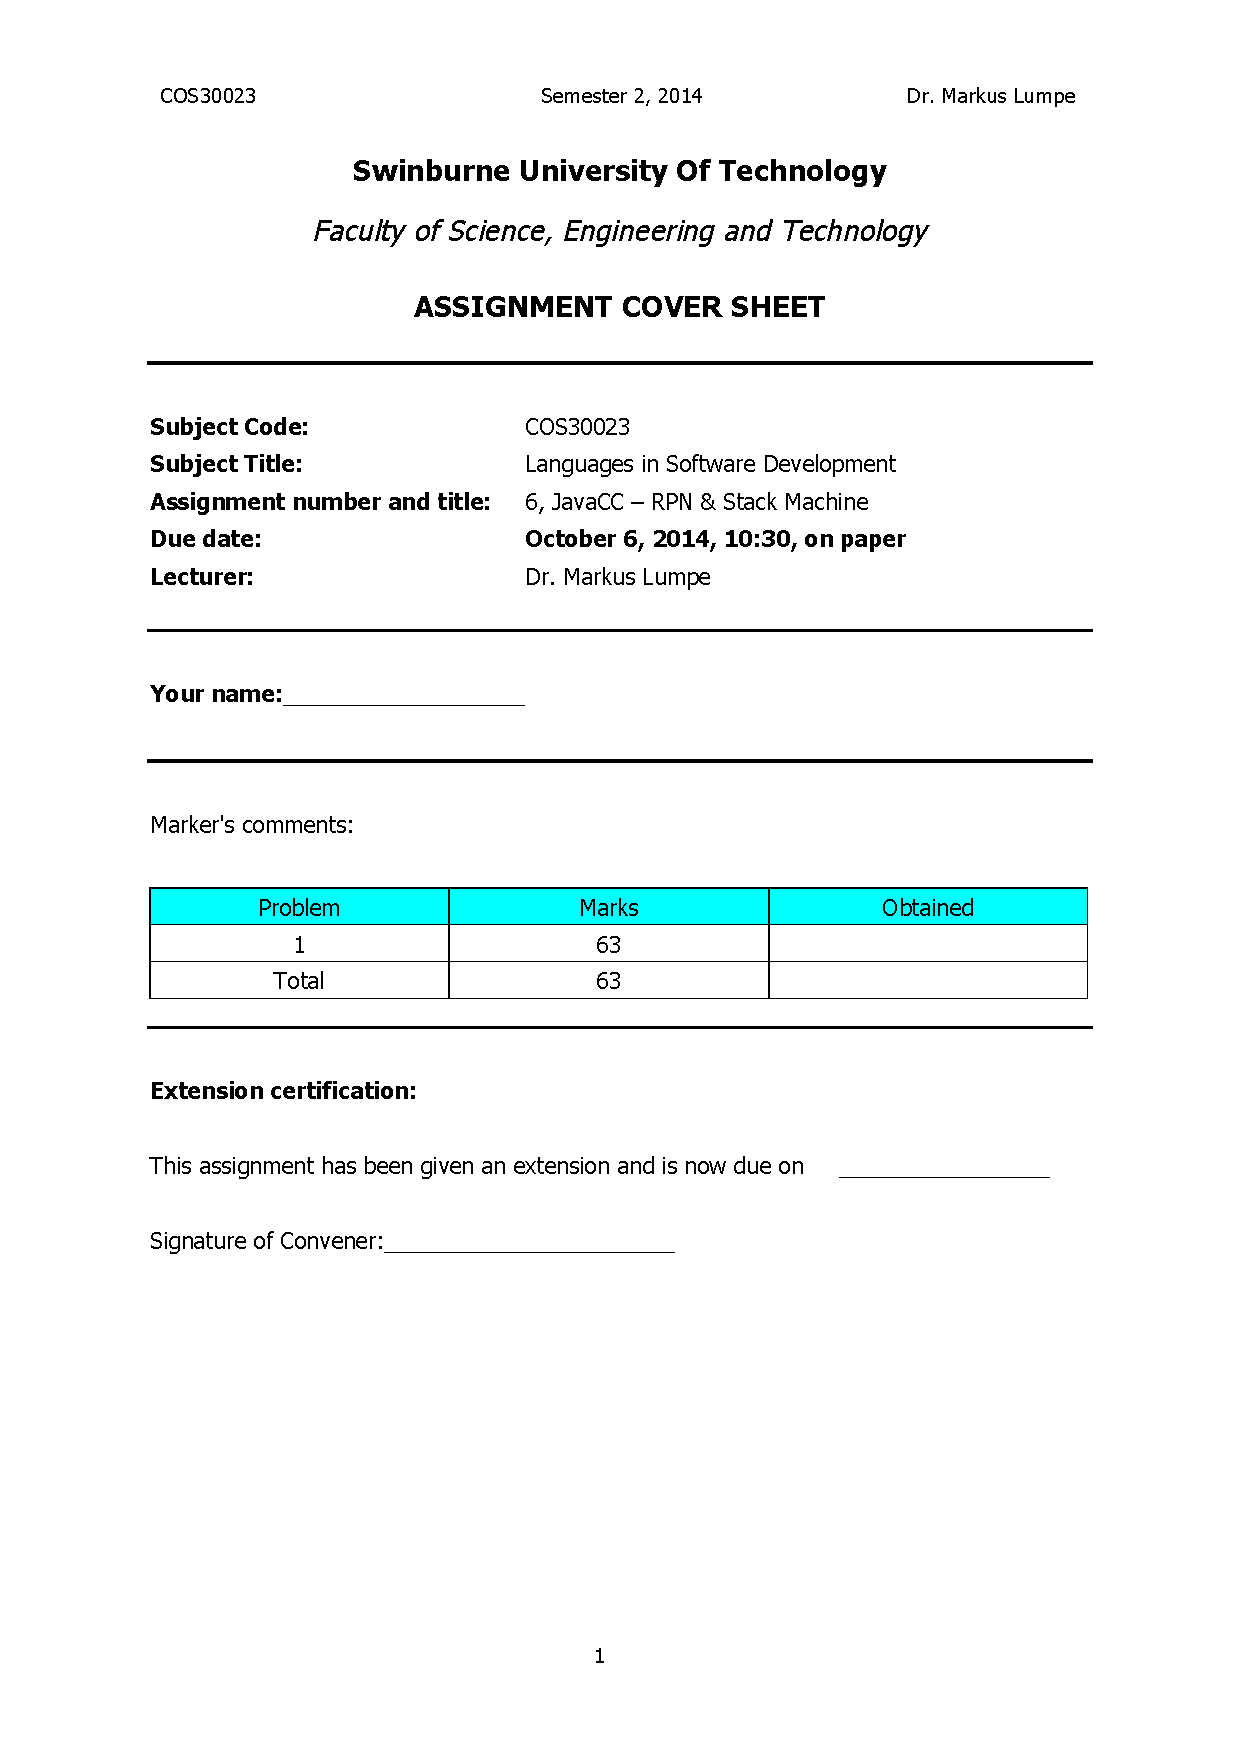
\includepdf[pages=1-1]{ProblemSet6.pdf}
\maketitle
\section{Parser and AST}
\subsection{Test Input}
\begin{minted}{nasm}
load 20.0
dup
store $a
load 4.0
load 2.0
mul
dup
print "4 * 2 = "
load 1.0
add
dup
print "4 * 2 + 1 = "
store $x
\end{minted}

\subsection{Result}
\begin{minted}{text}
PCode accepted:
load 20.0
dup
store $a
load 4.0
load 2.0
mul
dup
print "4 * 2 = "
load 1.0
add
dup
print "4 * 2 + 1 = "
store $x
Running program:
4 * 2 = 8.0
4 * 2 + 1 = 9.0
Stack:
1:	20.0
Memory:
$x:	9.0
$a:	20.0
\end{minted}

\begin{landscape}
\section{Source}
\subsubsection{PCodeParser.jj}
\inputminted{java}{RPN/src/PCodeParser.jj}

\subsubsection{ast.Position}
\inputminted{java}{RPN/src/ast/Position.java}
\subsubsection{ast.PCode}
\inputminted{java}{RPN/src/ast/PCode.java}
\subsubsection{ast.PCodeArgument}
\inputminted{java}{RPN/src/ast/PCodeArgument.java}

\subsubsection{ast.Add}
\inputminted{java}{RPN/src/ast/Add.java}
\subsubsection{ast.Sub}
\inputminted{java}{RPN/src/ast/Sub.java}
\subsubsection{ast.Mul}
\inputminted{java}{RPN/src/ast/Mul.java}
\subsubsection{ast.Div}
\inputminted{java}{RPN/src/ast/Div.java}
\subsubsection{ast.Dup}
\inputminted{java}{RPN/src/ast/Dup.java}

\subsubsection{ast.Load}
\inputminted{java}{RPN/src/ast/Load.java}
\subsubsection{ast.Store}
\inputminted{java}{RPN/src/ast/Store.java}
\subsubsection{ast.Print}
\inputminted{java}{RPN/src/ast/Print.java}

\subsubsection{ast.PCodeNumber}
\inputminted{java}{RPN/src/ast/PCodeNumber.java}
\subsubsection{ast.PCodeVariable}
\inputminted{java}{RPN/src/ast/PCodeVariable.java}

\subsubsection{machine.PCodeVisitor}
\inputminted{java}{RPN/src/machine/PCodeVisitor.java}
\subsubsection{machine.PCodeMachine}
\inputminted{java}{RPN/src/machine/PCodeMachine.java}

\end{landscape}
\end{document}
